\documentclass[twoside]{book}

% Packages required by doxygen
\usepackage{fixltx2e}
\usepackage{calc}
\usepackage{doxygen}
\usepackage[export]{adjustbox} % also loads graphicx
\usepackage{graphicx}
\usepackage[utf8]{inputenc}
\usepackage{makeidx}
\usepackage{multicol}
\usepackage{multirow}
\PassOptionsToPackage{warn}{textcomp}
\usepackage{textcomp}
\usepackage[nointegrals]{wasysym}
\usepackage[table]{xcolor}

% Font selection
\usepackage[T1]{fontenc}
\usepackage[scaled=.90]{helvet}
\usepackage{courier}
\usepackage{amssymb}
\usepackage{sectsty}
\renewcommand{\familydefault}{\sfdefault}
\allsectionsfont{%
  \fontseries{bc}\selectfont%
  \color{darkgray}%
}
\renewcommand{\DoxyLabelFont}{%
  \fontseries{bc}\selectfont%
  \color{darkgray}%
}
\newcommand{\+}{\discretionary{\mbox{\scriptsize$\hookleftarrow$}}{}{}}

% Page & text layout
\usepackage{geometry}
\geometry{%
  a4paper,%
  top=2.5cm,%
  bottom=2.5cm,%
  left=2.5cm,%
  right=2.5cm%
}
\tolerance=750
\hfuzz=15pt
\hbadness=750
\setlength{\emergencystretch}{15pt}
\setlength{\parindent}{0cm}
\setlength{\parskip}{3ex plus 2ex minus 2ex}
\makeatletter
\renewcommand{\paragraph}{%
  \@startsection{paragraph}{4}{0ex}{-1.0ex}{1.0ex}{%
    \normalfont\normalsize\bfseries\SS@parafont%
  }%
}
\renewcommand{\subparagraph}{%
  \@startsection{subparagraph}{5}{0ex}{-1.0ex}{1.0ex}{%
    \normalfont\normalsize\bfseries\SS@subparafont%
  }%
}
\makeatother

% Headers & footers
\usepackage{fancyhdr}
\pagestyle{fancyplain}
\fancyhead[LE]{\fancyplain{}{\bfseries\thepage}}
\fancyhead[CE]{\fancyplain{}{}}
\fancyhead[RE]{\fancyplain{}{\bfseries\leftmark}}
\fancyhead[LO]{\fancyplain{}{\bfseries\rightmark}}
\fancyhead[CO]{\fancyplain{}{}}
\fancyhead[RO]{\fancyplain{}{\bfseries\thepage}}
\fancyfoot[LE]{\fancyplain{}{}}
\fancyfoot[CE]{\fancyplain{}{}}
\fancyfoot[RE]{\fancyplain{}{\bfseries\scriptsize Generated by Doxygen }}
\fancyfoot[LO]{\fancyplain{}{\bfseries\scriptsize Generated by Doxygen }}
\fancyfoot[CO]{\fancyplain{}{}}
\fancyfoot[RO]{\fancyplain{}{}}
\renewcommand{\footrulewidth}{0.4pt}
\renewcommand{\chaptermark}[1]{%
  \markboth{#1}{}%
}
\renewcommand{\sectionmark}[1]{%
  \markright{\thesection\ #1}%
}

% Indices & bibliography
\usepackage{natbib}
\usepackage[titles]{tocloft}
\setcounter{tocdepth}{3}
\setcounter{secnumdepth}{5}
\makeindex

% Hyperlinks (required, but should be loaded last)
\usepackage{ifpdf}
\ifpdf
  \usepackage[pdftex,pagebackref=true]{hyperref}
\else
  \usepackage[ps2pdf,pagebackref=true]{hyperref}
\fi
\hypersetup{%
  colorlinks=true,%
  linkcolor=blue,%
  citecolor=blue,%
  unicode%
}

% Custom commands
\newcommand{\clearemptydoublepage}{%
  \newpage{\pagestyle{empty}\cleardoublepage}%
}

\usepackage{caption}
\captionsetup{labelsep=space,justification=centering,font={bf},singlelinecheck=off,skip=4pt,position=top}

%===== C O N T E N T S =====

\begin{document}

% Titlepage & ToC
\hypersetup{pageanchor=false,
             bookmarksnumbered=true,
             pdfencoding=unicode
            }
\pagenumbering{alph}
\begin{titlepage}
\vspace*{7cm}
\begin{center}%
{\Large Draph \\[1ex]\large 0.\+1.\+0 }\\
\vspace*{1cm}
{\large Generated by Doxygen 1.8.13}\\
\end{center}
\end{titlepage}
\clearemptydoublepage
\pagenumbering{roman}
\tableofcontents
\clearemptydoublepage
\pagenumbering{arabic}
\hypersetup{pageanchor=true}

%--- Begin generated contents ---
\chapter{Draph}
\label{index}\hypertarget{index}{}Dlang Facebook Graph A\+PI

Draph is a D language Facebook A\+PI that maps 1 to 1 the Facebook Graph A\+PI 
\chapter{Class Index}
\section{Class List}
Here are the classes, structs, unions and interfaces with brief descriptions\+:\begin{DoxyCompactList}
\item\contentsline{section}{\hyperlink{structevent_1_1event}{event\+::event} }{\pageref{structevent_1_1event}}{}
\item\contentsline{section}{\hyperlink{structlink_1_1Link}{link\+::\+Link} }{\pageref{structlink_1_1Link}}{}
\item\contentsline{section}{\hyperlink{structdraph_1_1Link}{draph\+::\+Link} }{\pageref{structdraph_1_1Link}}{}
\item\contentsline{section}{\hyperlink{structdraph_1_1User}{draph\+::\+User} }{\pageref{structdraph_1_1User}}{}
\item\contentsline{section}{\hyperlink{structuser_1_1User}{user\+::\+User} }{\pageref{structuser_1_1User}}{}
\end{DoxyCompactList}

\chapter{Class Documentation}
\hypertarget{structevent_1_1event}{}\section{event\+:\+:event Struct Reference}
\label{structevent_1_1event}\index{event\+::event@{event\+::event}}
\subsection*{Public Attributes}
\begin{DoxyCompactItemize}
\item 
\mbox{\Hypertarget{structevent_1_1event_a471112259b428c638465a85f483a5d9b}\label{structevent_1_1event_a471112259b428c638465a85f483a5d9b}} 
string {\bfseries id}
\item 
\mbox{\Hypertarget{structevent_1_1event_a96ee855e1d5a547d5577141664d172e4}\label{structevent_1_1event_a96ee855e1d5a547d5577141664d172e4}} 
int {\bfseries attending\+\_\+count}
\item 
\mbox{\Hypertarget{structevent_1_1event_aae1c82e5521067133900ef8e1f2d9335}\label{structevent_1_1event_aae1c82e5521067133900ef8e1f2d9335}} 
bool {\bfseries can\+\_\+guests\+\_\+invite}
\item 
\mbox{\Hypertarget{structevent_1_1event_acbaf7cb17407ec17f00c599612366120}\label{structevent_1_1event_acbaf7cb17407ec17f00c599612366120}} 
string {\bfseries category}
\item 
\mbox{\Hypertarget{structevent_1_1event_a90505c8b453a9d9321685c6bd4ee49b8}\label{structevent_1_1event_a90505c8b453a9d9321685c6bd4ee49b8}} 
Cover\+Photo {\bfseries cover}
\item 
\mbox{\Hypertarget{structevent_1_1event_a80752837fa9358ae86aa838accad315a}\label{structevent_1_1event_a80752837fa9358ae86aa838accad315a}} 
int {\bfseries declined\+\_\+count}
\item 
\mbox{\Hypertarget{structevent_1_1event_a7d13c9ef5c7c3b3cb67fecf6a6e9b54f}\label{structevent_1_1event_a7d13c9ef5c7c3b3cb67fecf6a6e9b54f}} 
string {\bfseries description}
\item 
\mbox{\Hypertarget{structevent_1_1event_ae1428217c8f98f8f660b1976b5fbfa0a}\label{structevent_1_1event_ae1428217c8f98f8f660b1976b5fbfa0a}} 
bool {\bfseries discount\+\_\+code\+\_\+enabled}
\item 
\mbox{\Hypertarget{structevent_1_1event_a9e390e9973ef960e9abb9ff043e581e6}\label{structevent_1_1event_a9e390e9973ef960e9abb9ff043e581e6}} 
string {\bfseries end\+\_\+time}
\item 
\mbox{\Hypertarget{structevent_1_1event_a0e02b6672629c7058d1bee0df8b09ff4}\label{structevent_1_1event_a0e02b6672629c7058d1bee0df8b09ff4}} 
Child\+Event \mbox{[}$\,$\mbox{]} {\bfseries event\+\_\+times}
\item 
\mbox{\Hypertarget{structevent_1_1event_af6b7df798a1f6722dc1ed6dd78cac867}\label{structevent_1_1event_af6b7df798a1f6722dc1ed6dd78cac867}} 
bool {\bfseries guest\+\_\+list\+\_\+enabled}
\item 
\mbox{\Hypertarget{structevent_1_1event_a2a09164fb85c3d7623f14ad6606e562d}\label{structevent_1_1event_a2a09164fb85c3d7623f14ad6606e562d}} 
int {\bfseries interested\+\_\+count}
\item 
\mbox{\Hypertarget{structevent_1_1event_abd861fd5918759b745bb185a191f8304}\label{structevent_1_1event_abd861fd5918759b745bb185a191f8304}} 
bool {\bfseries is\+\_\+canceled}
\item 
\mbox{\Hypertarget{structevent_1_1event_ad78f6b36a3ff3021f0ab10f12e36285a}\label{structevent_1_1event_ad78f6b36a3ff3021f0ab10f12e36285a}} 
bool {\bfseries is\+\_\+draft}
\item 
\mbox{\Hypertarget{structevent_1_1event_ad8e7a8d777b70691e0331ec8a7b16cbb}\label{structevent_1_1event_ad8e7a8d777b70691e0331ec8a7b16cbb}} 
bool {\bfseries is\+\_\+page\+\_\+owned}
\item 
\mbox{\Hypertarget{structevent_1_1event_a0fb90649bce5ca7324b1e9ea17dd428b}\label{structevent_1_1event_a0fb90649bce5ca7324b1e9ea17dd428b}} 
int {\bfseries maybe\+\_\+count}
\item 
\mbox{\Hypertarget{structevent_1_1event_ae9fd8fbe6ba4afaaf88d6c1ae6f1be4b}\label{structevent_1_1event_ae9fd8fbe6ba4afaaf88d6c1ae6f1be4b}} 
string {\bfseries name}
\item 
\mbox{\Hypertarget{structevent_1_1event_a4048967e71b40939b18c7da575a8afa0}\label{structevent_1_1event_a4048967e71b40939b18c7da575a8afa0}} 
int {\bfseries noreply\+\_\+count}
\item 
\mbox{\Hypertarget{structevent_1_1event_a2122cbc322df1583441cbd711a8765e6}\label{structevent_1_1event_a2122cbc322df1583441cbd711a8765e6}} 
Group {\bfseries parent\+\_\+group}
\item 
\mbox{\Hypertarget{structevent_1_1event_af924de79b010709b67c9037c0c03c13c}\label{structevent_1_1event_af924de79b010709b67c9037c0c03c13c}} 
Place {\bfseries place}
\item 
\mbox{\Hypertarget{structevent_1_1event_afb608d446566f23a3f553a1ce6bf07c4}\label{structevent_1_1event_afb608d446566f23a3f553a1ce6bf07c4}} 
string {\bfseries scheduled\+\_\+publish\+\_\+time}
\item 
\mbox{\Hypertarget{structevent_1_1event_a610358a5227fe1c780ea47d48ff39cc5}\label{structevent_1_1event_a610358a5227fe1c780ea47d48ff39cc5}} 
string {\bfseries start\+\_\+time}
\item 
\mbox{\Hypertarget{structevent_1_1event_abcc19bd08e52e3b6a5c9f6bdaea48227}\label{structevent_1_1event_abcc19bd08e52e3b6a5c9f6bdaea48227}} 
string {\bfseries ticket\+\_\+url}
\item 
\mbox{\Hypertarget{structevent_1_1event_adc40f87d95b525a795df369fc89212f8}\label{structevent_1_1event_adc40f87d95b525a795df369fc89212f8}} 
string {\bfseries ticket\+\_\+uri\+\_\+start\+\_\+sales\+\_\+time}
\item 
\mbox{\Hypertarget{structevent_1_1event_ac3367cbbf13e9e4c4d0de25b25f0fcf9}\label{structevent_1_1event_ac3367cbbf13e9e4c4d0de25b25f0fcf9}} 
string {\bfseries ticketing\+\_\+privacy\+\_\+uri}
\item 
\mbox{\Hypertarget{structevent_1_1event_a87d319fb6b4f1d3c972821c53e43af41}\label{structevent_1_1event_a87d319fb6b4f1d3c972821c53e43af41}} 
string {\bfseries ticketing\+\_\+terms\+\_\+uri}
\end{DoxyCompactItemize}


\subsection{Detailed Description}


Definition at line 3 of file event.\+d.



The documentation for this struct was generated from the following file\+:\begin{DoxyCompactItemize}
\item 
source/event.\+d\end{DoxyCompactItemize}

\hypertarget{structlink_1_1Link}{}\section{link\+:\+:Link Struct Reference}
\label{structlink_1_1Link}\index{link\+::\+Link@{link\+::\+Link}}
\subsection*{Public Attributes}
\begin{DoxyCompactItemize}
\item 
\mbox{\Hypertarget{structlink_1_1Link_a35d809fc4e6640fb4eeea74db780985d}\label{structlink_1_1Link_a35d809fc4e6640fb4eeea74db780985d}} 
string {\bfseries id}
\item 
\mbox{\Hypertarget{structlink_1_1Link_a5e2c852d064c31589b8d450e34f55762}\label{structlink_1_1Link_a5e2c852d064c31589b8d450e34f55762}} 
string {\bfseries created\+\_\+time}
\item 
\mbox{\Hypertarget{structlink_1_1Link_a21529a0f8e5cf20a3d41b1bc8e9bcc6d}\label{structlink_1_1Link_a21529a0f8e5cf20a3d41b1bc8e9bcc6d}} 
string {\bfseries description}
\item 
\mbox{\Hypertarget{structlink_1_1Link_af358a37c7b2487be48befd9902523e2e}\label{structlink_1_1Link_af358a37c7b2487be48befd9902523e2e}} 
User {\bfseries from}
\item 
\mbox{\Hypertarget{structlink_1_1Link_a3f6deef22f687fa9bf16429e2a4ff8ef}\label{structlink_1_1Link_a3f6deef22f687fa9bf16429e2a4ff8ef}} 
string {\bfseries icon}
\item 
\mbox{\Hypertarget{structlink_1_1Link_a685521716e1c70e478f173f0c34bb92b}\label{structlink_1_1Link_a685521716e1c70e478f173f0c34bb92b}} 
string {\bfseries link}
\item 
\mbox{\Hypertarget{structlink_1_1Link_ab35d8fe4cf111036a564719f69f565bb}\label{structlink_1_1Link_ab35d8fe4cf111036a564719f69f565bb}} 
string {\bfseries message}
\item 
\mbox{\Hypertarget{structlink_1_1Link_a461100dd85bd909bfd76b5901858996a}\label{structlink_1_1Link_a461100dd85bd909bfd76b5901858996a}} 
string {\bfseries name}
\item 
\mbox{\Hypertarget{structlink_1_1Link_ab6021020b07c54f0b29fe24586f44353}\label{structlink_1_1Link_ab6021020b07c54f0b29fe24586f44353}} 
string {\bfseries picture}
\end{DoxyCompactItemize}


\subsection{Detailed Description}


Definition at line 3 of file link.\+d.



The documentation for this struct was generated from the following file\+:\begin{DoxyCompactItemize}
\item 
source/link.\+d\end{DoxyCompactItemize}

\hypertarget{structdraph_1_1Link}{}\section{draph\+:\+:Link Struct Reference}
\label{structdraph_1_1Link}\index{draph\+::\+Link@{draph\+::\+Link}}


Collaboration diagram for draph\+:\+:Link\+:\nopagebreak
\begin{figure}[H]
\begin{center}
\leavevmode
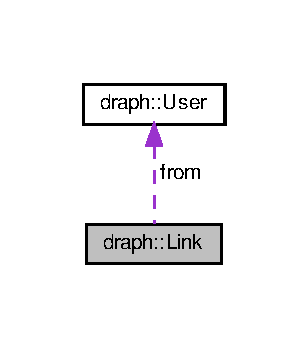
\includegraphics[width=148pt]{structdraph_1_1Link__coll__graph}
\end{center}
\end{figure}
\subsection*{Public Attributes}
\begin{DoxyCompactItemize}
\item 
\mbox{\Hypertarget{structdraph_1_1Link_ac8460919f97c36b46eb5c62e99f96391}\label{structdraph_1_1Link_ac8460919f97c36b46eb5c62e99f96391}} 
string {\bfseries id}
\item 
\mbox{\Hypertarget{structdraph_1_1Link_aacbe7ff208101a61c2970d0d37ab35e6}\label{structdraph_1_1Link_aacbe7ff208101a61c2970d0d37ab35e6}} 
string {\bfseries created\+\_\+time}
\item 
\mbox{\Hypertarget{structdraph_1_1Link_a4dfa15dc3f8328893015d73d77aac871}\label{structdraph_1_1Link_a4dfa15dc3f8328893015d73d77aac871}} 
string {\bfseries description}
\item 
\mbox{\Hypertarget{structdraph_1_1Link_a509a2f5acc4b37e71265bc6b38d9f966}\label{structdraph_1_1Link_a509a2f5acc4b37e71265bc6b38d9f966}} 
\hyperlink{structdraph_1_1User}{User} {\bfseries from}
\item 
\mbox{\Hypertarget{structdraph_1_1Link_afc96fffd750dd241c2db4d3aebb9762e}\label{structdraph_1_1Link_afc96fffd750dd241c2db4d3aebb9762e}} 
string {\bfseries icon}
\item 
\mbox{\Hypertarget{structdraph_1_1Link_a23be30f2ce181a49c68798fe63ce828b}\label{structdraph_1_1Link_a23be30f2ce181a49c68798fe63ce828b}} 
string {\bfseries link}
\item 
\mbox{\Hypertarget{structdraph_1_1Link_a988a5d092f47d398d376606a7f45c820}\label{structdraph_1_1Link_a988a5d092f47d398d376606a7f45c820}} 
string {\bfseries message}
\item 
\mbox{\Hypertarget{structdraph_1_1Link_a021587914f920f829813366b61f734f4}\label{structdraph_1_1Link_a021587914f920f829813366b61f734f4}} 
string {\bfseries name}
\item 
\mbox{\Hypertarget{structdraph_1_1Link_ae34bea53135fcfd05c27ce17be444bd8}\label{structdraph_1_1Link_ae34bea53135fcfd05c27ce17be444bd8}} 
string {\bfseries picture}
\end{DoxyCompactItemize}


\subsection{Detailed Description}


Definition at line 17 of file draph.\+d.



The documentation for this struct was generated from the following file\+:\begin{DoxyCompactItemize}
\item 
source/draph.\+d\end{DoxyCompactItemize}

\hypertarget{structdraph_1_1User}{}\section{draph\+:\+:User Struct Reference}
\label{structdraph_1_1User}\index{draph\+::\+User@{draph\+::\+User}}


\subsection{Detailed Description}


Definition at line 11 of file draph.\+d.



The documentation for this struct was generated from the following file\+:\begin{DoxyCompactItemize}
\item 
source/draph.\+d\end{DoxyCompactItemize}

\hypertarget{structuser_1_1User}{}\section{user\+:\+:User Struct Reference}
\label{structuser_1_1User}\index{user\+::\+User@{user\+::\+User}}


\subsection{Detailed Description}


Definition at line 3 of file user.\+d.



The documentation for this struct was generated from the following file\+:\begin{DoxyCompactItemize}
\item 
source/user.\+d\end{DoxyCompactItemize}

%--- End generated contents ---

% Index
\backmatter
\newpage
\phantomsection
\clearemptydoublepage
\addcontentsline{toc}{chapter}{Index}
\printindex

\end{document}
